\documentclass{article}
\usepackage{hyperref}
\usepackage{graphicx} % Required for inserting images

\title{\textbf{ASSIGNMENT-4 \\ BATEMAN EQUATION}}
\author{Barath.S.D \\ MM22B002}

\begin{document}

\maketitle
\section{MM22B002}
\subsection{Introduction}
In nuclear physics, the Bateman equation is a mathematical model describing abundances and activities in a decay chain as a function of time, based on the decay rates and initial abundances. The model was formulated by Ernest Rutherford in 1905 and the analytical solution was provided by Harry Bateman in 1910.
\subsection{The equation}
If, at time t, there are N\textsc{i}(t) atoms of isotope i that decays into isotope i+1 at a rate $\lambda$\textsc{i} the amounts of isotopes in the k-step decay chain evolves as: 
\newline{}
\newline{}
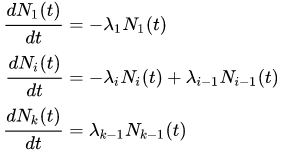
\includegraphics[width=8cm]{image1.png}
\subsection{Applications}
This can be adapted to handle decay branches). While this can be solved explicitly for i = 2, the formulas quickly become cumbersome for longer chains.
The Bateman equation is a classical master equation where the transition rates are only allowed from one species (i) to the next (i+1) but never in the reverse sense (i+1 to i is forbidden). \newline{}
\newline{}
For example, for the simple case of a chain of three isotopes the corresponding Bateman equation reduces to \newline{} \newline{}
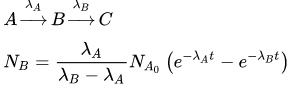
\includegraphics[width=5cm]{image.png}
\newline{}
\begin{enumerate}
    \item\textbf{NAME : BARATH.S.D}
    \item\textbf{ROLL NO. : MM22B002}
    \item\textbf{GITHUB USERNAME : BARATH-SD \\ USER ID : 135802163}
\end{enumerate}
\footnote{\url{https://en.wikipedia.org/wiki/Bateman_equation}}

\end{document}
